\documentclass[mla7]{mla}
\usepackage{amsmath}
\graphicspath{ {./images/} }

\title{An Exploration of Path Tracking on a Small Nonholonomic Robot}
\author{Joseph Spencer}
\professor{Mr. Taddiken, Mr. Miserendino}
\course{McMullen Capstone 903}
\date{17 September 2020} 

\begin{document}

\begin{paper}

\section{Follow-The-Carrot}
Follow-the-Carrot is one of the simplest forms of path tracking. It gives no control over the linear velocity of the vehicle and seeks only to make the robot face a selected point along the path, called the goal point or carrot point. It functions with the idea that facing a point on the path ahead of the vehicle while driving forward will keep the vehicle sufficiently close to the path.

This method first selects the carrot point by finding a point that is both on the path and a predefined distance, called the lookahead distance, from the vehicle. Using this point and the position of the vehicle, the target heading is calculated as the heading of the line pointing from the vehicle to the carrot point. The error $e_0$ can then be calculated as the difference between the target heading and the actual heading:
\begin{equation}
 e_0 = \text{atan2}(y_2 - y_1,x_2 - x_1) - \theta
\end{equation}
in which the point $(x_1,y_1)$ is the position of the vehicle, $\theta$ is the vehicle's heading, and the point $(x_2,y_2)$ is the carrot point.

This error then governs the angular velocity of the vehicle, causing it to turn towards the target heading. This can be done in two ways, either through a proportional gain (Lundgren) or a full PID controller (Hogg et al.). In the former method, the error is simply multiplied by a scalar $k_p$, called the proportional gain, then assigned to the desired angular velocity of the vehicle $\phi$:
\begin{equation}
\phi = k_p * e_0
\end{equation}

However, to improve the performance of this controller, one can use a PID controller. A PID controller, instead of only considering the error at the current moment of time, considers the error itself (P), as well as the integral (I) and derivative (D) of the error with respect to time. It follows that each of these terms has its own gain value, $k_p$, $k_i$, and $k_d$, respectively, to form the following equation:
\begin{equation}
\phi = k_p e_0 + k_i \int_0^t \! e(\tau) \, d\tau + k_d \frac{de(t)}{dt}
\end{equation}

Using a PID controller instead of only a proportional term can add additional stability to the system. The integral term works to remove stead state error, or small errors that do not reduce to zero over time, usually caused by the motors not operating under a certain voltage. The derivative term works to prevent overshoot by dampening the control signal if the error approaches zero too quickly. Both additional control values usually help make the system more easily controllable.

However, both versions of the Follow-the-Carrot algorithm are not necessarily effective. As Lundgren says, ``the vehicle has a tendency to naturally cut corners'' (Lundgren 3). This is because as soon as a carrot point is selected around the corner, the vehicle will attempt to turn towards it, usually before the vehicle has reached the corner. Lundgren also claims that the vehicle could oscillate over the path. While the testing of Hogg et al. showed this effect to be minimal when using the PID method, it is likely a significant issue for the proportional method.

The nature of this algorithm is like an inverted pendulum, as the vehicle is always moving forward, any small error in the heading is magnified as the vehicle moves. While a control system such as this can control an inherently unstable system like an inverted pendulum, the instability that is introduced is not ideal for the algorithm's performance.

\section{Pure Pursuit}

The pure pursuit algorithm is one of the oldest and most popular algorithms in the field of path tracking, known for its robustness. It was first introduced into the field of path tracking, having previously been used only for literal pursuit, in Dr. Wallace's "First Results in Robot Road-Following" and later popularized in Dr. Coulter's "Implementation of the Pure Pursuit Path Tracking Algorithm."

Pure Pursuit follows a similar procedure to Follow-the-Carrot in its goal point selection, choosing a point on the path that is a specified distance from the vehicle. However, rather than an error function and gains approach, Pure Pursuit uses a more geometric system. Once a goal point has been determined, a circle is found that passes through both the position of the vehicle and the goal point, as well as being tangent to the heading of the vehicle (see fig. 1). This circle, therefore, describes a path from the current position of the robot to the goal point which requires the robot to drive with a constant curvature. This curvature becomes the control output from the algorithm.

\begin{figure}[H]
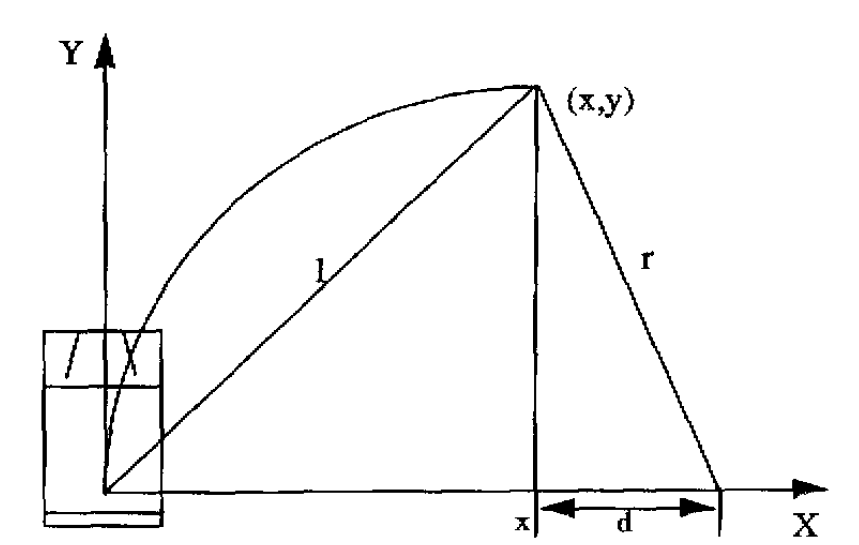
\includegraphics[width=0.4\linewidth]{CoulterPurePursuitDiagram}
\captionsetup{justification=centering,margin=2cm}
\caption{Geometry of Pure Pursuit Algorithm from: Coulter, R. Craig. “Implementation of the Pure Pursuit Path Tracking Algorithm.” p. 5}
\label{img:pp1}
\end{figure}

Note that in fig. \ref{img:pp1}, the point $(x,y)$ corresponds to the goal point in the local coordinates of the vehicle. The curvature of the circle $\gamma$, as derived by Coulter, can be calculated as follows:
\begin{subequations}
\begin{align}
d&=r-x \\
(r-x)^2+y^2&=r^2 \\
r^2-2rx+x^2+y^2&=r^2 \\
2rx&=l^2 \\
r&=\frac{l^2}{2x} \\
\gamma &= \frac{2x}{l^2}
\end{align}
\end{subequations}
 Then, the curvature needs to be converted into angular velocity:
\begin{subequations}
\begin{align}
\gamma &= \frac{d\theta}{ds} \\
\gamma * \frac{ds}{dt} &= \frac{d\theta}{ds} * \frac{ds}{dt} \\
\gamma * v &= \omega
\end{align}
\end{subequations}
And so, the faster the vehicle is moving, the more aggressively the vehicle will react to curvature.

Additionally, notice how the only parameter which can be tuned is the lookahead distance for the goal point. As an added benefit to the algorithm, this makes it much easier to tune than other algorithms with many tuning parameters. Note: more will be added here later but I wanted to give some attention to the other algorithms

\section{The Stanley Method}

The Stanley Method of path tracking was developed by the Stanford Racing Team's entry in the 2005 DARPA Grand Challenge, an offroad autonomous automotive race (Hoffmann et al.). Given the offroad nature of the conditions this vehicle was expected to face, the algorithm has proved robust, especially following large disturbances. Hoffmann et al. claimed the algorithm was able to produce results of "a typical root mean square (RMS) crosstrack error of under 0.1 m" (Hoffmann et al. 1). Crosstrack here refers to the distance between the path and the vehicle, so a low value of crosstrack error corresponds to accurate tracking of the path.

Unlike the previous methods, the Stanley Method does not use a lookahead distance, and instead looks at the point closest to the robot. The primary motivation for doing this is to put a significant part of the controller's effort into aligning itself with the path. From this nearest point, it uses the heading of the point (or tangent direction of the path at the point), the distance from the point to the vehicle's position, as well as the vehicle's velocity. As a car was used in the original vehicle, note that the output of the controller is the angle to which the wheels are turned in an Ackerman steering mechanism. Additionally, more factors, such as a dampening gain for the inertia of the wheels' steering direction turning have been removed for the purposes of this paper, as they are not relevant to the skid-steer drive tested here. The original control law is as follows:
\begin{equation}
\delta(t)=\Psi(t)+\arctan{\frac{ke(t)}{v(t)}}
\end{equation}
where $\delta$ is the steering angle, $\Psi$ is the difference between the vehicle's heading and the nearest point's heading, $k$ is a gain, $e$ is the crosstrack error, and $v$ is the velocity.
The steering angle can then be converted to curvature (denoted $\gamma$ here), and the curvature can be converted to angular momentum:
\begin{subequations}
\begin{align}
\delta(t)&=\Psi(t)+\arctan{\frac{ke(t)}{v(t)}} \\
\gamma(t)&=\frac{1}{l}\tan{(\Psi(t)+\arctan{\frac{ke(t)}{v(t)}})} \label{eqn:stanley22}\\
\omega(t)&=\frac{v(t)}{l}\tan{(\Psi(t)+\arctan{\frac{ke(t)}{v(t)}})} \label{eqn:stanley23}
\end{align}
\end{subequations}
in equations \ref{eqn:stanley22} and \ref{eqn:stanley23}, $l$ represents the distance between the front and rear wheels of Ackerman steering type vehicle that the skid-steer robot using this algorithm will be emulating. In this context, it will be considered a tuning variable.

The findings of outside sources reflect well on this algorithm. Hoffmann et al. explain that the algorithm is mathematically proven to cause the vehicle to converge to the path exponentially, suggesting a high degree of robustness (4). Pendleton et al. claim that ``Compared to the pure pursuit method, the Stanley method, has better tracking results and does not cut corners'' (30). They attribute this to the use of crosstrack error as opposed to pursuit. However, Pendleton et al. also state that the Stanley method may behave similarly to a Pure Pursuit controller with a small lookahead distance, that is to say, it oscillates over the path (31). This behavior is undesirable, as causes the robot to move an excessive distance not in the direction of the path, slowing down the system, as well as giving the path planner less control over the vehicle's motion, which could be potentially dangerous to the vehicle or the surrounding environment.

\section{Follow the Past}

Follow the Past is a unique path tracking algorithm developed by Dr. Hellström of Umeå University, Sweden, that instead of following a mathematically defined path, it attempts to drive the vehicle along a recorded path, as driven by a human driver. It was also designed for use with a robot for articulated steering, so the output signal corresponds to a steering angle. Like the Stanley Method, the relationship between the steering angle $\phi$ and the curvature $\kappa$ is:
\begin{equation}
\kappa=\frac{1}{l}\tan{\phi}
\end{equation}
for a tunable value $l$ which corresponds to the distance between the wheel and the articulation point.

The algorithm determines the steering angle based on three behavior values desired by the controller: $\phi_\beta$, which turns towards the recorded heading, $\phi_\gamma$, which mimics the recorded steering angle, and $\phi_\alpha$, which turns towards the desired position along the path. $\phi_\beta$ and $\phi_\gamma$ are defined trivially:
\begin{subequations}
\begin{align}
\phi_\beta &= \theta^\prime-\theta \\
\phi_\gamma &= \phi^\prime
\end{align}
\end{subequations}
where $\theta^\prime$ and $\phi^\prime$ are the recorded heading and steering angle at the nearest point.

$\phi_\alpha$ is defined via two methods in Ringdahl and Hellström's paper; the latter will be used here as the original authors state that it is less susceptible to oscillations than the former. In this method, a look ahead point is defined that is a distance $l$ ahead of the path point nearest to the vehicle, in the direction $\theta^\prime+\phi^\prime$ (see fig. \ref{img:ftp1}). $\psi$ is then defined as the heading from the vehicle to the look ahead point. Finally, $\phi_\alpha=\psi-\theta^\prime-\phi^\prime$, such that $\phi_\alpha$ is the difference in heading from the path point to the look ahead point, and the heading from the vehicle position to the look ahead point. This provides a control value that works to move the vehicle back onto the path, without risking oversaturating the controller if lateral error grows to large, as $\phi_\alpha$ is inherently bounded between $(-\frac{\pi}{2},\frac{\pi}{2})$.

\begin{figure}[H]
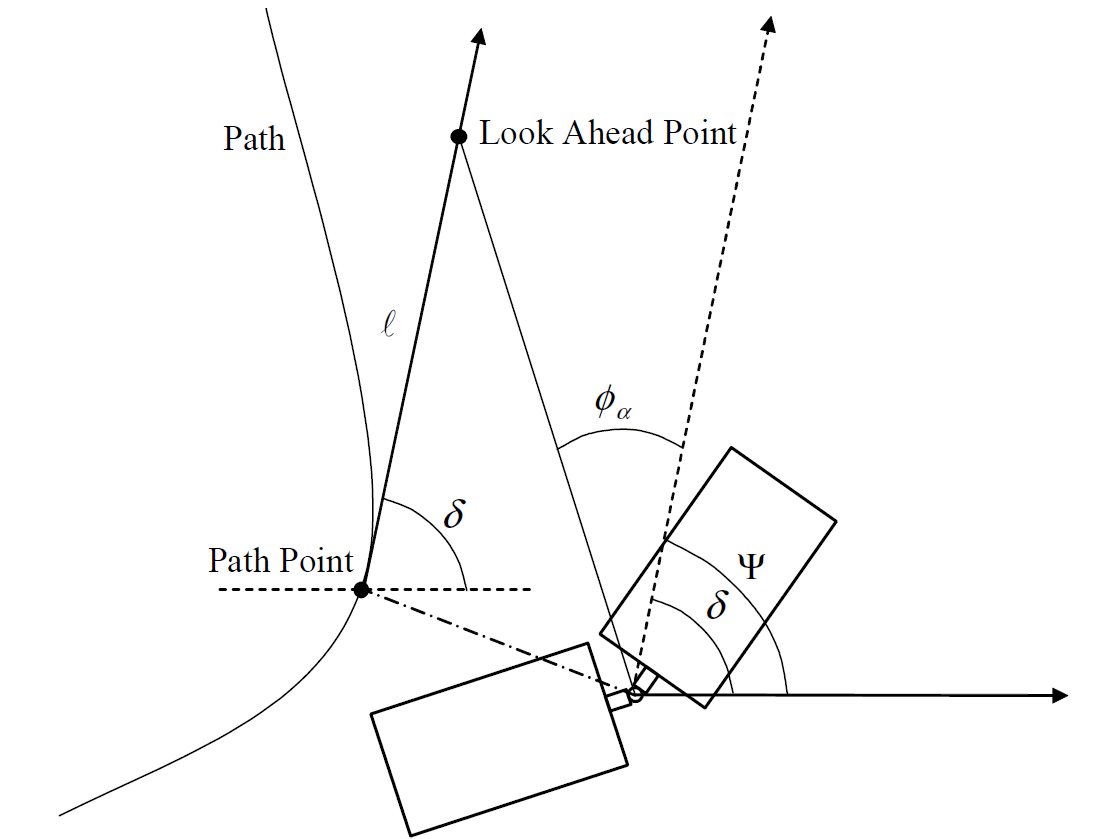
\includegraphics[width=0.5\linewidth]{RingdahlFtPDiagram}
\captionsetup{justification=centering,margin=2cm}
\caption{Geometry of Follow the Past Algorithm from: Ringdahl, Ola, and Thomas Hellström. “Follow the Past - A Path Tracking Method Using Recorded Orientation and Steering Commands.” p. 5}
\label{img:ftp1}
\end{figure}

\section{Vector Pursuit}

Vector Pursuit is a path tracking method created by Dr. Jeffrey Wit, which describes a desired transformation of the vehicle using Screw Theory, in a similar way to Pure Pursuit's use of arcs.

Screws are described by a centerline and a pitch; when combined with an angular movement, it describes the angular and positional transformation on any rigid body. The centerline of such a screw can be defined by a set of Plücker line coordinates. Plücker line coordinates consist of two vectors, $(\vec{S}\,; \vec{S}_0)$, the first of which is parallel to the center line with unit length, and the second of which is defined as:
\begin{equation}
\vec{S}_0=\vec{r} \times \vec{S} \label{eqn:vector1}
\end{equation}
for any $\vec{r}$ which lies on the center line. Screw Theory takes this further by adding a pitch component $h$, and lets the Plücker coordinates be referred to by a single symbol $\vec{\$}$:
\begin{equation}
\vec{\$}=(\vec{S}\,; \vec{r} \times \vec{S} + h\vec{S}) = (\vec{S}\,; \vec{S}_{0h})
\end{equation}

The advantage of using this representation is that putting the screw in local coordinates of a rigid body, such that the rigid body is at $(0,0)$, $\omega\vec{S}_{0h}$ is the instantaneous velocity of the rigid body around the screw. Additionally, if the pitch of the screw tends towards infinity, the screw models a pure translation in the direction of $\vec{S}$; for a velocity $v$, the screw simplifies to:
\begin{equation}
v\vec{\$}=(\vec{0}\,; v\vec{S})
\end{equation}
as Wit says, it ``is a screw that has a centerline at infinity" (44). The intuition for this is lies in equation \ref{eqn:vector1}; as a zero vector cross a point on the centerline is a finite vector, it follows that every point on the line must have an infinite magnitude.

For the implementation of Vector Pursuit, Dr. Wit considers two methods, however only the second will be considered for this paper, as it better handles the nonholonomic constraints of the skid-steer testing robot and had better results in Dr. Wit's own testing. In this implementation, it initially follows similarly to other geometric path tracking methods, in that it selects a goal point that is on the path that is one lookahead distance away from the vehicle. However, unlike those algorithms, Vector Pursuit takes the heading at the goal point into consideration.

The basis of the algorithm is to generate a screw that corrects the translational error, $\vec{\$}_t$, and another screw that corrects the orientation error, $\vec{\$}_r$, and add them together to create a target screw. Each of these screws are defined by the following:
\begin{subequations}
\begin{align}
\vec{\$}_t&=k_t\left( 0,0,1\,; ^W\!y_v+\frac{d^2}{2\,^V\!y_L}\cos{\theta_v}, -^W\!x_v+\frac{d^2}{2\,^V\!y_L}\sin{\theta_v}, 0 \right) \text{if\,} ^V\!y_L\neq0 \\
\vec{\$}_t&=k_t\left( 0,0,0\,; \frac{^W\!x_L-^W\!x_V}{d}, \frac{^W\!y_L-^W\!y_L}{d}, 0 \right) \text{if\,} ^V\!y_L=0 \\
\vec{\$}_r&=k_r\left( 0,0,1\,; ^W\!y_v, -^W\!x_v, 0 \right)
\end{align}
\end{subequations}
in which $k_t$ and $k_r$ are gains, $d$ is the lookahead distance, $(^W\!x_v,^W\!y_v)$ and $\theta_v$ are the position and heading of the vehicle $(^W\!x_L,^W\!y_L)$ is the position of the goal point, and $^V\!y_L$ is the distance from the vehicle to the goal point, only in the vehicle's lateral direction (Wit 57). When these screws are combined, they yield:
\begin{subequations}
\begin{multline}
\vec{\$}_d=\left( 0,0,k_t+k_r\,; k_r\,^W\!y_v + k_t \left( ^W\!y_v+\frac{d^2}{2\,^V\!y_L}\cos{\theta_v} \right), \right. \\ \left. -k_r\,^W\!x_v + k_t \left( -^W\!x_v+\frac{d^2}{2\,^V\!y_L}\sin{\theta_v} \right), 0 \right) \text{if\,} ^V\!y_L\neq0
\end{multline}
\begin{multline}
\vec{\$}_d=\left( 0,0,k_r\,; k_r\,^W\!y_v + k_t \left( \frac{^W\!x_L-^W\!x_V}{d} \right), \right. \\ \left. -k_r\,^W\!x_v + k_t \left( \frac{^W\!y_L-^W\!y_L}{d} \right), 0 \right) \text{if\,} ^V\!y_L=0
\end{multline}
\end{subequations}

After summing the two screws, the gains $k_t$ and $k_r$ are determined by a desired relative proportion $k$ between the amount of time needed to reach the translational target and the amount of time needed to reach the orientation target. For example, if $k=1$, the algorithm will move the vehicle such that if the motion was sustained, each target would be met at the same time. This allows tuning based on whether position or orientation should be emphasized by the controller. Upon the substitution of this relationship, the center of $\vec{\$}_d$, $(^W\!x_{\vec{\$}_d}, ^W\!y_{\vec{\$}_d})$ can be calculated. The distance between the center of the screw and the vehicle is the radius, and from that the curvature of the desired motion can be calculated. These coordinates simplify to:
\begin{subequations}
\begin{align}
^W\!x_{\vec{\$}_d} &=^W\!x_v - \frac{k\phi}{(k-1)\phi+(\theta_L-\theta_v)} \left( \frac{d^2}{2\,^V\!y_L}\cos{\theta_v} \right)\\
^W\!y_{\vec{\$}_d} &=^W\!y_v - \frac{k\phi}{(k-1)\phi+(\theta_L-\theta_v)} \left( \frac{d^2}{2\,^V\!y_L}\sin{\theta_v} \right)
\text{if\,}^V\!y_L\neq0 \text{, or}\\
^W\!x_{\vec{\$}_d} &= ^W\!x_v - k \left( \frac{^W\!y_L-^W\!y_v}{\theta_L-\theta_v} \right) \\
^W\!y_{\vec{\$}_d} &= ^W\!y_v - k \left( \frac{^W\!x_L-^W\!x_v}{\theta_L-\theta_v} \right) 
\text{if\,} ^V\!y_L=0
\end{align}
\end{subequations}
these variables mean the same as used in previous equations, as well as $\phi$ being the angle between the vehicle position and the goal point from the perspective of the centerline of the screw $\vec{\$}_d$.  This finally is used to calculate the radius of the screw by:
\begin{equation}
r= -^W\!x_v\sin{\theta_v}+^W\!y_v\cos{\theta_v}-\left(-^W\!x_{\vec{\$}_d}\sin{\theta_v}+^W\!y_{\vec{\$}_d}\cos{\theta_v}\right)
\end{equation}
Similar to other methods, once the desired radius is found, it can be converted into a desired angular velocity. In this case, $\omega$ is:
\begin{equation}
\omega=\frac{v_{current}}{r}
\end{equation}

Multiple sources praise the Vector Pursuit method for its robustness and effectiveness. Wit, the original author claimed that the algorithm``was less sensitive to the chosen look-ahead distance at various speeds [than Pure Pursuit and Follow-the-Carrot], and it was able to handle situations ... after an unexpected obstacle was encountered'' (108). Lundgren echoes the importance of this, stating that such cases occur in the real world, when a ``vehicle detects sudden obstacles appearing on the path,'' or ``if there is noise in the position estimations, which can happen if the vehicle was using GPS techniques for localizing'' (Lundgren 7).

\end{paper}

\end{document}